\section{Theorie}
\label{sec:Theorie}

Ein Trägheitsmoment ist immer bezüglich einer Achse definiert, um die sich das zu beobachtende Objekt dreht.
Dreht sich ein ausgedehnter Körper um eine feste Achse, so dreht sich jedes einzelne Massenelement $m_i$ des Körpers
und es folgt das Gesamtträgheitsmoment des Körpers zu

\begin{equation*}
    \label{eqn:traegheitsm}
    I = \sum_i r_i^2 \cdot m_i.
\end{equation*}

\noindent
Dabei ist $r_i$ der Abstand des i-ten Massenelements $m_i$ senkrecht zur Drehachse.
Für unendlich viele infinitesimal kleine Massenelemente geht die Gleichung \autoref{eqn:traegheitsm} in die Relation 

\begin{equation}
    \label{eqn:traegheitsmoment}
    I = \int r_{\perp}^2 \, dm
\end{equation}

\noindent
über.
Für die Beschreibung komplexerer Körper, wird der beschriebene Körper in einzelne Teilkörper aufgeteilt. Das Gesamtträgheitsmoment ergibt
sich dann als die Summe der Trägheitsmomente der Teilkörper. Dabei ist darauf zu achten, dass alle aufsummierten Körper sich auf die 
gleiche Achse beziehen.
Ist die Drehachse nicht gleich der Schwerpunktsache des Körpers, so liefert der \textit{Steiner'sche Satz} einen Weg zur Berechnung des
Trägheitsmomentes $I$

\begin{equation}
    \label{eqn:steiner}
    I = I_{\text{S}} \, + m a^2,
\end{equation}

\noindent
sofern die beiden Achsen parallel zueinander sind.
Dabei ist $I_{\text{S}}$ das Trägheitsmoment des Körpers bei Drehung um die Schwerpunktsache, $m$ die Masse des Körpers und $a$ der 
Abstand der Schwerpunktsache zur Drehachse. 
\noindent
Wirkt auf einen Körper im Abstand $\vec r$ eine Kraft $\vec F$, so wirkt auf ihn ein \textit{Drehmoment}, was wie folgt defieniert ist.

\begin{equation*}
    \label{eqn:drehmoment}
    \vec M = \vec F\times\vec r
\end{equation*}

\noindent
Eine Spiralfeder, wie sie auch an der Apparatur in dem Versuch angebracht ist, verrichtet ein Drehmoment, das der Auslenkung entgegengerichtet ist.
Es folgt damit der Zusammenhang.
\begin{equation}
    \label{eqn:winkelrichtgr}
    \vec M = -D \vec\varphi    
\end{equation} 
Dabei ist $D$ die Winkelrichtgröße, beziehungsweise der Proportionalitätsfaktor
und $\vec\varphi$ der Auslenkwinkel \cite{gerthsen}.
Unter einer solchen Voraussetzung führt der Körper eine harmonische Schwingung aus, dessen Periodendauer wie folgt lautet.

\begin{equation}
    \label{eqn:periode}
    T=2\pi\sqrt\frac{I}{D}.
\end{equation}

Aus \autoref{eqn:traegheitsmoment} folgen die Trägheitsmomente für  einfache Körper, die \autoref{fig:traegheitsbsp} zu entnehmen sind
\begin{align}
    I_{\text{Stab}} = \frac{1}{12} ml^2, \label{eqn:Istab} \\
    I_{\text{Kugel}} = \frac{2}{5} mR^2, \label{eqn:IKugel} \\
    I_{\text{Zylinder}} = \frac{1}{2} mR^2, \label{eqn:Izylinder} \\
    I_{\text{zh}} = m (\frac{r^2}{4} +\frac{h^2}{12}). \label{eqn:Izh}
\end{align}

\begin{figure}[H]
    \centering
    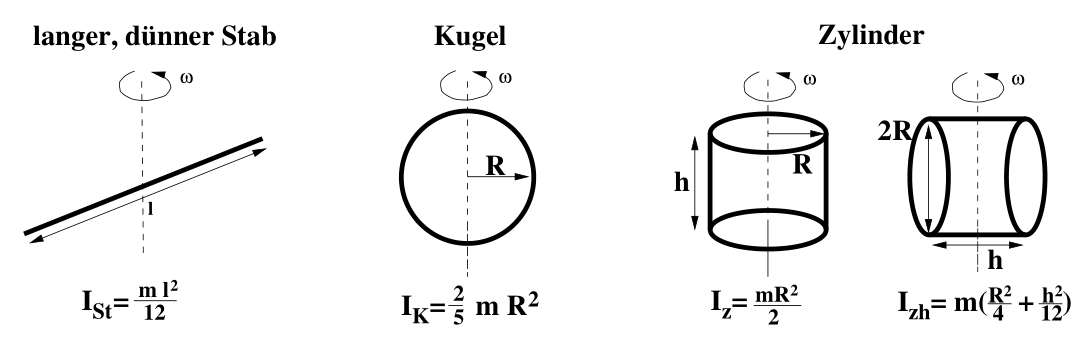
\includegraphics[width=0.75\textwidth]{Bilder/traegheitsbeispiele.png}
    \caption{Trägheitsmomente einfacher Körper \cite{Anleitung}.}
    \label{fig:traegheitsbsp}
  \end{figure}